\newcommand{\pointing}{\includegraphics[width=1em]{assets/point.png}}
\begin{itemize}
    \item \textbf{Náhodná veličina} -- číselné vyjádření výsledku náhodného pokusu.
    \item Základní typy NV -- \textbf{diskrétní} NV, \textbf{spojitá} NV.
    \item \textbf{Rozdělení pravděpodobnosti} -- Předpis, který jednoznačně určuje všechny pravděpodobnosti typu $P(X \in M)$, kde $M \subset \mathbb{R}$

          (tj. $P (X = a), P (X < a), P(X > a), P(a < X < b), ...,$ kde $a, b \in \mathbb{R}$).
          \begin{itemize}
              \item Rozdělení pravděpodobnosti \textbf{DNV} -- distribuční funkcí $F(x) = P(X < x),$ resp. \textbf{pravěpodobnostní funkcí} $P(x_i)$.
              \item Rozdělení pravděpodobnosti \textbf{SNV} -- distribuční funkcí $F(x) = P(X < x),$ resp. \textbf{hustotou pravěpodobnostní} $f(x)$.
          \end{itemize}
    \item \textbf{Číselné charakteristiky pro popis NV} -- střední hodnota $\mathbf{E(X)}$, rozptyl $\mathbf{D(X)}$, směrodatná odchylka $\mathbf{\sigma(X)}$, p--kvantily $\mathbf{x_p}$
\end{itemize}

\section{Diskrétní náhodná veličina}
\textit{Příklady}
\begin{itemize}
    \item[$\circ$] počet šroubů typu M10 mezi 10 vybranými (víme-li, že do dodávky 100 šroubů bylo omylem zařazeno 20 šroubů typu M50)
    \item[$\circ$] počet pacientů (z 10 očkovaných) u nichž byla použita prošlá očkovací látka (víme-li, že v balení bylo 20 dávek očkovací látky, přičemž 5 z nich bylo prošlých)

          \begin{itemize}
              \item[$\rhd$] \textbf{Obecně:} -- počet úspěchů v $n$ (závislých) pokusech
          \end{itemize}
    \item[$\circ$] počet správně přenesených bitů předtím než dojde ke $4.$ chybě (víme-li, že pravděpodobnost chybného přenosu bitu je $0,12$)
    \item[$\circ$] počet dobrovolníků, které budeme muset testovat dříve než najdeme 5 dárců s krevní skupinou AB (předpokládejme, že dobrovolníci neznají svou krevní skupinu, pravděpodobnost výskytu krevní skupiny (populační frekvence) krevní skupiny AB je $0,05$)
          \begin{itemize}
              \item[$\rhd$] \textbf{Obecně:} -- počet (nezávislých) pokusů do $k.$ úspěchu
          \end{itemize}
    \item[$\circ$] počet škrábanců na $1 m^2$ lakovaného povrchu (víme-li, že průměrně lze očekávat 3 škrábance na $10 m^2$)
    \item[$\circ$] počet červených krvinek v $10 ml$ krve ženy (víme-li, že u průměrně lze pozorovat $4,8 \cdot 10^{12}$ červených krvinek v $1l$ krve (u žen))
          \begin{itemize}
              \item[$\rhd$] \textbf{Obecně:} -- počet událostí v časovém intervalu, na ploše, v objemu
          \end{itemize}
\end{itemize}
\subsection{Bernoulliho pokusy}
\begin{itemize}
    \item \textbf{Posloupnost nezávislých pokusů majících pouze dva možné výsledky} (takových pokusů, kdy úspěch v libovolné skupině pokusů neovlivňuje pravděpodobnost úspěchů v pokusu, který do této skupiny nepatří).
    \item \textbf{v nichž jev A} (úspěch) \textbf{nastává s pravděpodobností } $\mathbf{\pi}$ a neúspěch s pravděpodobností $1 - \pi$.
\end{itemize}

\textit{Příklad:} Předpokládejme, že pravděpodobnost narození dívky je $0,49$. Jaká je pravděpodobnost toho, že mezi čtyřmi dětmi v rodině je právě jedna dívka?
\begin{itemize}
    \item X… počet dívek mezi 4 dětmi
    \item D ... narodí se dívka, $P(D) = \pi$
    \item $\bar{D}$ ...  narodí se kluk, $P(D) = 1 - \pi$
\end{itemize}
\begin{equation*}
    \begin{split}
        &(X = 1) \,... \, \{D\bar{D}\bar{D}\bar{D},\bar{D}D\bar{D}\bar{D},\bar{D}\bar{D}D\bar{D},\bar{D}\bar{D}\bar{D}D\} \\
        &P(D\bar{D}\bar{D}\bar{D}) = P(\bar{D}D\bar{D}\bar{D}) = P(\bar{D}\bar{D}D\bar{D}) = P(\bar{D}\bar{D}\bar{D}D) = \pi \cdot (1 - \pi)^3 \\
        &P(X = 1) = P(D\bar{D}\bar{D}\bar{D} \cup \bar{D}D\bar{D}\bar{D} \cup \bar{D}\bar{D}D\bar{D} \cup \bar{D}\bar{D}\bar{D}D) = \binom{4}{1} \cdot \pi \cdot (1 - \pi)^3 \\
        &P(X = 1) = 0,260
    \end{split}
\end{equation*}

\subsection{Binomické rozdělení}
\begin{itemize}
    \item \textbf{X .. počet úspěchů v $n$ Bernoulliho pokusech} $$X \sim Bi(n;\pi)$$ \\ $n$ -- počet pokusů \\ $\pi$ -- pravděpodobnost úspěchu
          \begin{figure}[H]
              \centering
              \includegraphics[width=0.8\textwidth]{assets/12_binom}
          \end{figure}
    \item \textbf{Střední hodnota}: $\qquad$ $E(X) = n\pi$
    \item \textbf{Rozptyl}: $\qquad\qquad\qquad\;\; D(X) = n\pi(1 - \pi)$
    \item Vlastnosti
          \begin{figure}[H]
              \centering
              \includegraphics[width=0.5\textwidth]{assets/12_binom_vlast}
              \caption{$\pi \not= 0,5$, s rostoucím $n$ se rozdělení stává více a více symetrickým}
          \end{figure}
          \begin{figure}[H]
              \centering
              \includegraphics[width=0.5\textwidth]{assets/12_binom_vlast2}
          \end{figure}
    \item[$\circ$] \textit{Příklad} Mezi 200 vajíčky určenými pro prodej v jisté maloobchodní prodejně je 50 vajíček prasklých. Jaká je pravděpodobnost, že vybereme--li si náhodně 20 vajec, bude 8 z nich prasklých?
          \begin{itemize}
              \item $X$ … počet prasklých vajec z 20 vybraných (výběr bez vracení)

                    \begin{center}
                        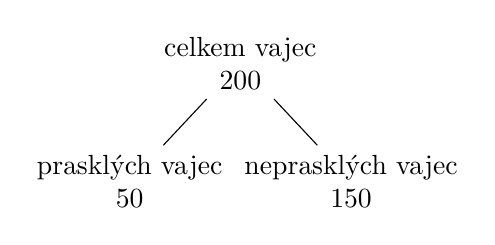
\begin{tikzpicture}[sibling distance=8em,
                                every node/.style = { align=center,
                                        top color=white, bottom color=white}]]
                            \node {celkem vajec\\200}
                            child { node {prasklých vajec\\50} }
                            child { node {neprasklých vajec\\150} };
                        \end{tikzpicture}
                    \end{center}
                    $$P(X = 8) = \frac{\binom{50}{8} \binom{150}{12}} {\binom{200}{20}}$$
              \item[] \textbf{počet příznivých možností} -- vybíráme 8 prasklých z 50 prasklých a zároveň 12 ze 150 neprasklých \\ \textbf{počet všech možností }-- vybíráme 20 vajec z 200
          \end{itemize}
\end{itemize}

\subsection{Hypergeometrické rozdělení}
\begin{itemize}
    \item \textbf{ $\mathbf{X}$ ... počet prvků se sledovanou vlastností ve výběru $n$ prvků}
    \item V souboru \textbf{N} prvků je \textbf{M} s danou vlastností a zbylých (\textbf{N -- M}) prvků tuto vlastnost nemá. Postupně vybereme ze souboru \textbf{n} prvků, z nichž žádný \textbf{nevracíme zpět}.
          $$X \sim H(N;M;n)$$ \\ $N$ -- rozsah základního souboru \\ $M$ -- počet prvků s danou vlastností \\ $n$ -- rozsah výběru
    \item \textbf{Pravděpodobnostní funkce}: $P(X = k) = \frac {\mathbin{\color{blue} \binom{M}{k} \binom{N-M}{n-k}}} {\mathbin{\color{magenta}\binom{N}{n}}}$
          \begin{itemize}
              \item \textcolor{blue}{Počet příznívých možností, tj. počet možností jak vybrat $k$ prvků s danou vlastností z $M$ a zároveň $(n-k)$ prvků, které uvedenou vlastnost nemají z $(N - M)$ prvků.}
              \item \textcolor{magenta}{Počet všech možností, jak vybrat $n$ prvků z $N$ (nezáleží na pořadí).}
          \end{itemize}
    \item \textbf{Střední hodnota}: $\qquad$ $E(X) = n \cdot \frac{M}{N}$
    \item \textbf{Rozptyl}: $\qquad\qquad\qquad\;\; D(X) = n \cdot \frac{M}{N}(1 - \frac{M}{N})(\frac{N-n}{N-1})$
    \item \textbf{Možnost aproximace} -- je--li $n/N$, tzv. \textbf{výběrový poměr}, menší než $0,05$, lze hypergeometrické rozdělení nahradit binomickým s parametry $n$ a $M/N$. $$(\frac{n}{N} < 0,05) \Rightarrow [H(N;M;n) \approx Bi(n;\frac{M}{N})]$$
\end{itemize}

\subsection{Negativně binomické (Pascalovo) rozdělení}
\begin{itemize}
    \item \textbf{$X$ ... počet Bernoulliho pokusů do $k.$ výskytu události (úspěchu), včetně $k.$ výskytu}
          $$X \sim NB(k;\pi)$$ \\ $k$ -- požadovaný počet úspěchů (výskytu události) \\ $\pi$ -- pravděpodobnost úspěchu
    \item \textbf{Pravděpodobnostní funkce:}
          \begin{figure}[H]
              \centering
              \includegraphics[width=0.7\textwidth]{assets/12_neg_binom}
          \end{figure}
    \item \textbf{Střední hodnota}: $\qquad$ $E(X) = \frac{k}{\pi}$
    \item \textbf{Rozptyl}: $\qquad\qquad\qquad\;\; D(X) = \frac{k(1- \pi)}{\pi^2}$
    \item V případě negativně binomické náhodné veličiny není definice ustálená. Někteří statistici (popř. statistický software) ji definují jako \textbf{počet neúspěchů před $k.$ úspěchem}.
\end{itemize}

\subsection{Poissonův proces}
\textbf{Bodový proces}
\begin{itemize}
    \item Sledujeme chod procesu, v němž čas od času dochází k nějaké význačné události \\
          \begin{figure}[H]
              \centering
              \includegraphics[width=0.5\textwidth]{assets/12_poisson_proces}
          \end{figure}
    \item Registrujeme počet událostí $N(s;t)$ v časovém intervalu $<s;s + t>$
    \item \textbf{Rychlost výskytu události $\lambda$} je parametrem Poissonova procesu
    \item Poissonův proces lze obdobně jako v časovém intervalu definovat na libovolné uzavřené prostorové oblasti (na ploše, v objemu).
\end{itemize}
Jako \textbf{Poissonův proces} označujeme proces, který je:
\begin{itemize}
    \item \textbf{ordinální} -- pravděpodobnost výskytu více než jedné události v limitně krátkém časovém intervalu $(t \to 0)$ je nulová. (tzv. \textbf{řídké jevy}),
    \item \textbf{stacionální} -- rychlost výskytu událostí $\lambda$ je konstantní v průběhu sledovaného intervalu,
    \item \textbf{beznásledný} -- pravděpodobnost výskytu událostí není závislá na čase, který uplynul od minulé události.
\end{itemize}

\subsection{Poissonovo rozdělení}
\begin{itemize}
    \item \textbf{$X$ ... počet výskytu události v uzavřené oblasti (v čase, na ploše, v objemu)}
    \item náhodný pokus jako Poissonův proces (nezávislé události probíhající v čase $t$, s rychlostí výskytu $\lambda$; popř. nezávislé události objevující se na ploše $t$, resp. v objemu $t$ s hustotou výskytu $\lambda$).
          $$X \sim Po(\lambda t)$$
    \item \textbf{Pravděpodobnostní funkce}: $P(X = k) = \frac{(\lambda t)^k}{k!}e^{-\lambda t}$
    \item \textbf{Střední hodnota}: $\qquad$ $E(X) = \frac{k}{\pi}$
    \item \textbf{Rozptyl}: $\qquad\qquad\qquad\;\; D(X) = \frac{k(1- \pi)}{\pi^2}$
\end{itemize}


\section{Spojitá náhodná veličina}
\begin{itemize}
    \item Hustota pravděpodobnosti f(x) -- funkce $f(x)$ je \textbf{hustotou pravděpodobnosti} (na intervalu $a \leq x \leq b$), jestliže splňuje následující podmínky:
          \begin{itemize}
              \item $f(x) \geq 0; x \in \mathbb{R}$
              \item plocha pod křivkou hustoty je rovna 1 ($\int_{-\infty}^{\infty} f(x)dx = 1$).
          \end{itemize}
\end{itemize}

\subsection{Exponenciální rozdělení}
\begin{itemize}
    \item \textbf{$X$ ... délka časových intervalů mezi událostmi v Poissonově procesu}
          $$X \sim Exp(\lambda)$$
    \item Předpokládá konstantní intenzitu události $\lambda(t)$- rozdělení \uv{bez paměti}.
    \item \textbf{Hustota pravděpodobnosti}:
          $f(t) =  \begin{cases}
                  \lambda \cdot e^{-\lambda t} & \quad t > 0     \\
                  0,                           & \quad t \leq 0.
              \end{cases}$
    \item \textbf{Distribuční funkce}:
          $\qquad\qquad F(t) =  \begin{cases}
                  1 -  e^{-\lambda t} & \quad t > 0     \\
                  0,                  & \quad t \leq 0.
              \end{cases}$
    \item \textbf{Střední hodnota}: $\qquad\qquad\quad E(X) = \frac{1}{\lambda}$
    \item \textbf{Rozptyl}: $\qquad\qquad\qquad\qquad\quad D(X) = (E(X))^2 = \frac{1}{\lambda^2}$ \\
    \item \textbf{Riziková funkce} (intenzita poruch) $\lambda (t)$
          \begin{itemize}
              \item Pro nezápornou náhodnou veličinu $X$ se spojitým rozdělením popsaným distribuční funkcí $F(t)$ definujeme pro $F(t) \not= 1$ rizikovou funkci jako  $$\lambda(t) = \frac{f(t)}{1 - F(t)}.$$
              \item $\lambda(t)$ -- Představuje-li náhodná veličina X dobu do poruchy nějakého zařízení, pak pravděpodobnost, že pokud do času t nedošlo k žádné poruše, tak k ní dojde v následujícím krátkém úseku délky $\Delta t$, je přibližně
                    $$P(t \geq X <t + \Delta t|X > t) = \lambda(t) \cdot \Delta t$$
                    \begin{figure}[H]
                        \centering
                        \includegraphics[width=0.5\textwidth]{assets/12_exp_rizk_fce}
                    \end{figure}
              \item[$\circ$] \textit{Příklad} Střední doba čekání zákazníka na obsluhu v prodejně je 50 sekund. Doba čekání se řídí exponenciálním rozdělením (pravděpodobnost, že zákazník nebude obsloužen klesá s rostoucím časem exponenciálně). Jaká je pravděpodobnost, že náhodný zákazník bude obsloužen dříve než za 30 sekund?
                    \begin{itemize}
                        \item[] X -- doba čekání na obsluhu
                        \item[] $X \sim Exp (\lambda = \frac{1}{50}s^-1), E(X) = \frac{1}{\lambda} = 50 s$
                    \end{itemize}
          \end{itemize}
\end{itemize}

\subsection{Weibullovo rozdělení}
\begin{itemize}
    \item \textbf{X ... délka časových intervalů mezi událostmi v Poissonově procesu}
    \item Zobecnění exponenciálního rozdělení
    \item Tímto rozdělením lze modelovat i dobu do výskytu události u systémů (jedinců), které jsou v období dětských nemocí, resp. období stárnutí.
          $$X \sim W(\theta;\beta)$$
          \\ $\theta$ -- parametr měřítka (scale) $\theta = \frac{1}{\lambda}; \theta > 0$ \\ $\beta$ -- parametr tvaru (shape); $\beta > 0$
    \item \textbf{Hustota pravděpodobnosti}:
          $f(t) =  \begin{cases}
                  \beta\lambda^{\beta} t^{\beta-1}e^{-(\lambda t)^{\beta}}, & \quad t > 0     \\
                  0,                                                        & \quad t \leq 0.
              \end{cases}$
    \item \textbf{Distribuční funkce}:
          $\qquad\qquad F(t) =  \begin{cases}
                  1 -  e^{-(\lambda t)^{\beta} } & \quad t > 0     \\
                  0,                             & \quad t \leq 0.
              \end{cases}$
    \item \textbf{Riziková funkce}:
          $\qquad\qquad\quad\; \lambda(t) =  \begin{cases}
                  \beta\lambda^\beta t^{\beta-1} & \quad t > 0     \\
                  0,                             & \quad t \leq 0.
              \end{cases}$
          \begin{figure}[H]
              \centering
              \includegraphics[width=0.5\textwidth]{assets/12_weib_riz_fce}
              \caption{Riziková funkce}
          \end{figure}
\end{itemize}
\subsection{Normální rozdělení}
\begin{itemize}
    \item Bývá vhodné k popisu náhodných veličin, které lze interpretovat jako aditivní výsledek mnoha nepatrných a vzájemně nezávislých faktorů (výška člověka, IQ, délka končetiny).
    \item Popisuje náhodné veličiny, jejichž hodnoty se symetricky shlukují kolem střední hodnoty a vytvářejí tak charakteristický tvar hustoty pravděpodobnosti známý pod názvem \textbf{Gaussova křivka}. $$X \sim N (\mu;\sigma^2)$$  \\$\mu$ -- střední hodnota \\ $\sigma^2$ -- rozptyl
    \item \textbf{Hustota pravděpodobnosti}: $f(x) = \frac{1}{\sigma \sqrt{2\pi}} e^{-\frac{1}{2}({\frac{x - \mu}{\sigma}})^2}$
          \begin{figure}[H]
              \centering
              \includegraphics[width=0.5\textwidth]{assets/12_norm_roz}
              \caption{Riziková funkce}
          \end{figure}
    \item \textbf{Distribuční funkce}: $F(x) = \frac{1}{\sigma \sqrt{2\pi}} \int_{-\infty}^{x} e^{-\frac{1}{2}(\frac{t - \mu}{\sigma})^2} dt$\\ (integrál nelze řešit analyticky)
\end{itemize}

%BTICH END